\chapter{Esperimenti svolti}
Una serie di esperimenti è stata condotta al fine di valutare l'efficacia del sistema proposto nella compressione video applicata alle light field images.

\section{Applicazione del sistema proposto sui dataset utilizzati in precedenza}
Inizialmente sono stati eseguiti una serie di test utilizzando il nostro sistema per valutare le prestazioni dei dataset precedenti. Ciò ha consentito di ottenere una comprensione più approfondita delle dinamiche operative e dei risultati ottenuti dai nostri precedessori, permettendoci, inoltre, di identificare fino a quale punto il sistema precedente ha risposto alle esigenze previste.
L'obiettivo principali è stato quello di valutare con maggiore precisione l'efficacia delle metodologie utilizzate precedentemente e di identificare eventuali punti deboli o aree di miglioramento. 

\section{Studio sulla correlazione tra light field contigui}
Al fine di valutare l'impatto dell'ordine dei frames nei dataset originali, è stato condotto uno studio supplementare. Ogni dataset originale è stato sottoposto a un processo di trasformazione, generando così un nuovo dataset in cui i frames sono disposti in maniera casuale. 
L'obiettivo di questo studio è comprendere come la disposizione casuale dei frames influenzi le prestazioni e i risultati dei codec di compressione. Tale approccio è fondamentale per valutare la resilienza dei codec di compressione rispetto a variazioni nell'ordine temporale dei frames. 

\section{Aggiunta di nuovi codec e nuovi dataset}
La scelta di aggiungere nuovi codec e di sottoporre tutti i dataset, vecchi e nuovi, a un riesame completo è stata fondamentale per comprendere in maniera esaustiva come le nuove implementazioni influiscano sulle prestazioni complessive del sistema. Tale approccio ha consentito di identificare correlazioni significative tra le caratteristiche dei codec, la selezione del dataset e le performance globali, contribuendo a delineare un quadro completo delle dinamiche del sistema in esame.


\subsection{Dataset utilizzati}
Per il miglioramento dello studio già effettuato dai nostri colleghi, abbiamo deciso di utilizzare i 3 dataset implementati nel loro progetto, in modo da poterli testare su nuovi codec, in aggiunta a 7 ulteriori dataset. Lo scopo è di avere un confronto tra più dati, in modo da raggiungere risultati più accurati.
\\
\\
I dadaset aggiunti sono i seguenti:
\begin{itemize}
    \item Il dataset ”Messerschmitt”\cite{Messerschmitt}, realizzato dal MIT Media Lab, propone 25 immagini in formato .png rappresentanti scene renderizzate, Figura\ref{fig:Messerschmitt}. Esse mostrano modelli 3D di una vettura del marchio Messerschmitt  realizzati dallo Stanford University Computer Graphics Laboratory \cite{3Dscanrep}. Tutti i light fields hanno una risoluzione di 840 x 593 pixel.
    
    \item Il dataset ”Dice”\cite{Dice}, realizzato dal MIT Media Lab, propone 25 immagini in formato .png rappresentanti scene renderizzate, Figura \ref{fig:Dice}. Esse mostrano modelli 3D di dadi da gioco realizzati dallo Stanford University Computer Graphics Laboratory \cite{3Dscanrep}. Tutti i light fields hanno una risoluzione di 840 x 593 pixel.
    
    \item Il dataset ”Fish”\cite{Fish}, realizzato dal MIT Media Lab, propone 25 immagini in formato .png rappresentanti scene renderizzate, Figura \ref{fig:Fish}. Esse mostrano modelli 3D pesci realizzati dallo Stanford University Computer Graphics Laboratory \cite{3Dscanrep}. Tutti i light fields hanno una risoluzione di 840 x 593 pixel.

    \item  Il dataset ”Car”\cite{Car} realizzato dal Max Planck Institut Informatik. Esso consiste in 101 immagini in formato .png, rappresentanti scene renderizzate, Figura \ref{fig:Car}. Esse presentano scene 3D di una autovettura. Tutti i light fields hanno una risoluzione spaziale di 960 x 720 pixel

    \item  Il dataset ”Cobblestone”\cite{Cobblestone} realizzato dal Max Planck Institut Informatik. Esso consiste in 101 immagini in formato .png, rappresentanti scene renderizzate, Figura \ref{fig:Cobblestone}. Esse presentano scene 3D di un sentiero di pietra. Tutti i light fields hanno una risoluzione spaziale di 960 x 720 pixel

    \item  Il dataset ”Mannequin”\cite{Mannequin} realizzato dal Max Planck Institut Informatik. Esso consiste in 101 immagini in formato .png, rappresentanti scene renderizzate, Figura \ref{fig:Mannequin}. Esse presentano scene 3D di un manichino in una stanza. Tutti i light fields hanno una risoluzione spaziale di 960 x 720 pixel

    \item  Il dataset ”Blob”\cite{Blob} realizzato dal Max Planck Institut Informatik. Esso consiste in 101 immagini in formato .png, rappresentanti scene renderizzate, Figura \ref{fig:Blob}. Esse presentano scene 3D di un "blob". Tutti i light fields hanno una risoluzione spaziale di 960 x 720 pixel


\end{itemize}


\begin{figure}[ht]
    \centering
    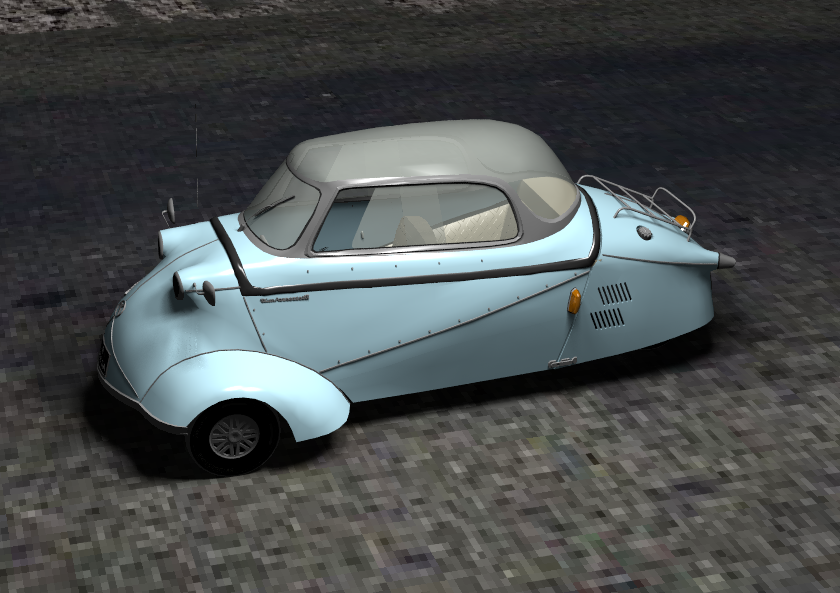
\includegraphics[width=0.5\textwidth]{img/Messerschmitt.png}
    \caption{Immagine estratta dal dataset ”Messerschmitt”}
    \label{fig:Messerschmitt}
\end{figure}

\begin{figure}[ht]
    \centering
    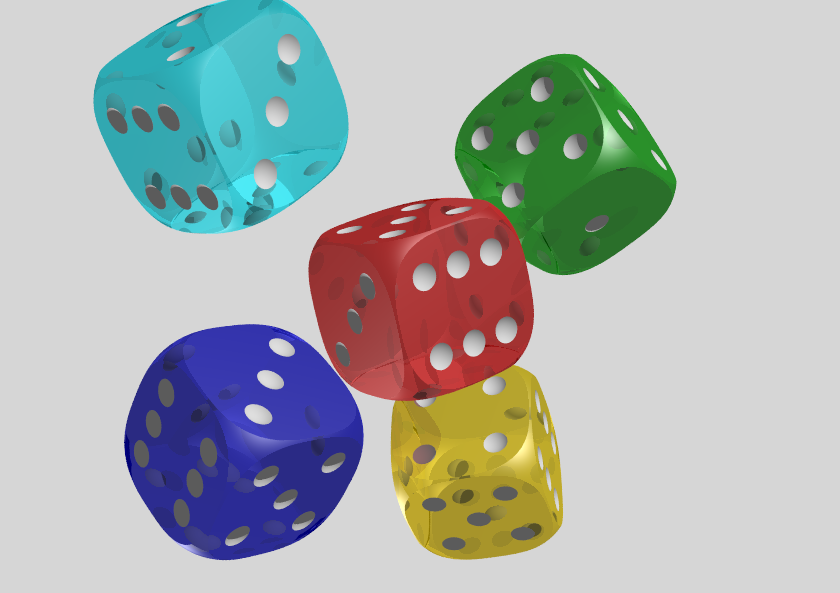
\includegraphics[width=0.5\textwidth]{img/Dice.png}
    \caption{Immagine estratta dal dataset ”Dice”}
    \label{fig:Dice}
\end{figure}

\begin{figure}[ht]
    \centering
    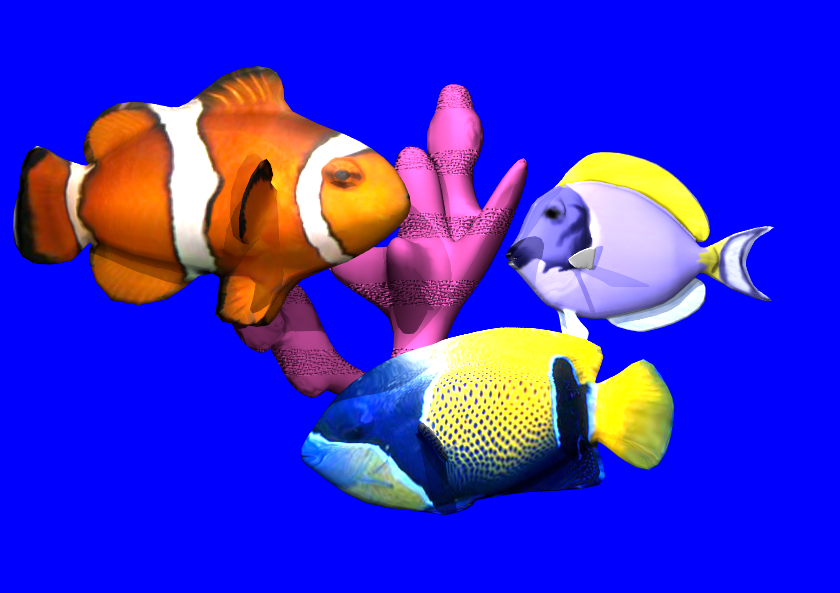
\includegraphics[width=0.5\textwidth]{img/Fish.png}
    \caption{Immagine estratta dal dataset ”Fish”}
    \label{fig:Fish}
\end{figure}

\begin{figure}[ht]
    \centering
    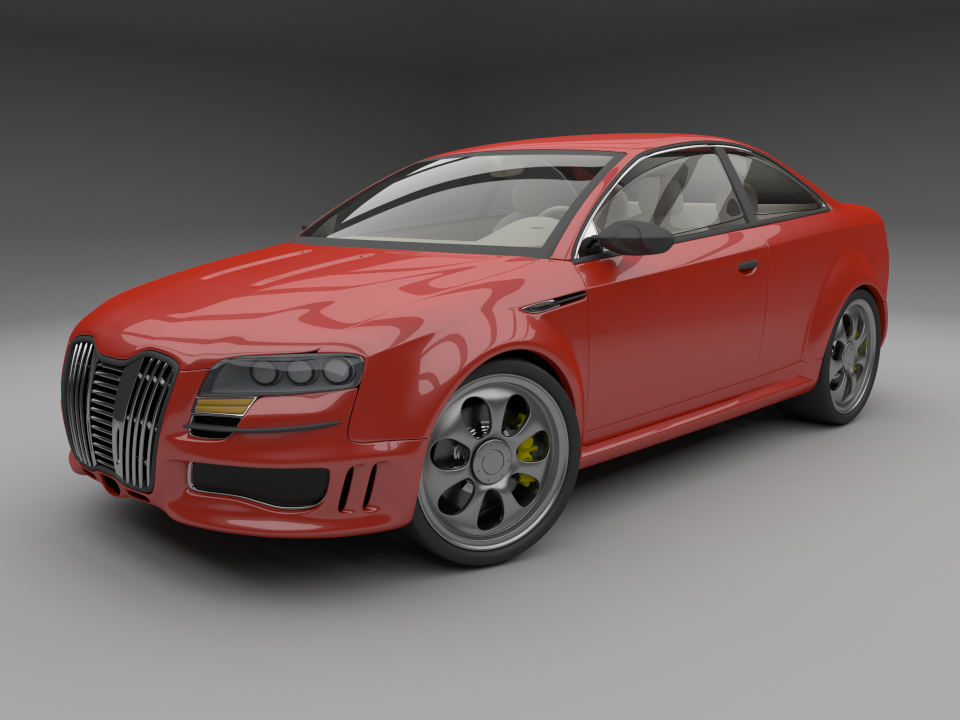
\includegraphics[width=0.5\textwidth]{img/Car.png}
    \caption{Immagine estratta dal dataset ”Car”}
    \label{fig:Car}
\end{figure}

\begin{figure}[ht]
    \centering
    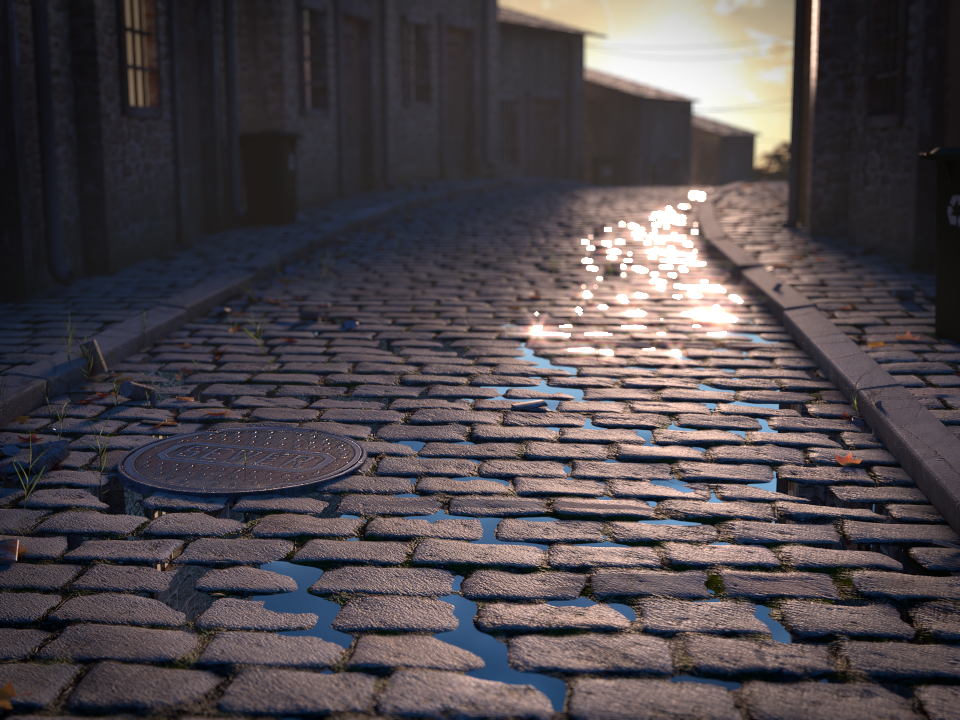
\includegraphics[width=0.5\textwidth]{img/Cobblestone.png}
    \caption{Immagine estratta dal dataset ”Cobblestone”}
    \label{fig:Cobblestone}
\end{figure}

\begin{figure}[ht]
    \centering
    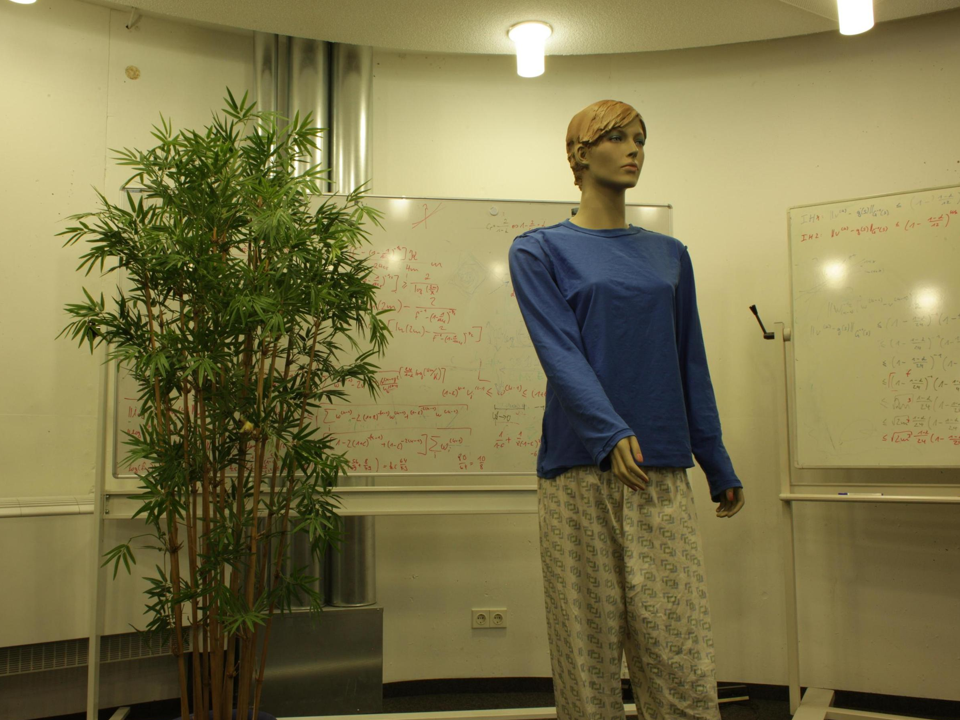
\includegraphics[width=0.5\textwidth]{img/Mannequin.png}
    \caption{Immagine estratta dal dataset ”Mannequin”}
    \label{fig:Mannequin}
\end{figure}

\begin{figure}[ht]
    \centering
    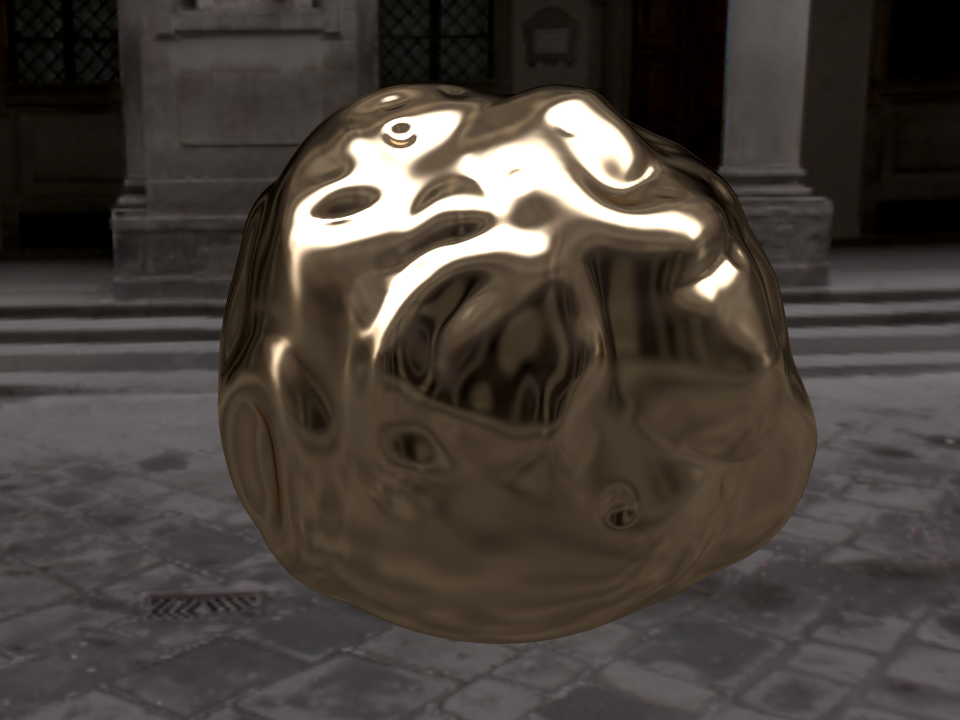
\includegraphics[width=0.5\textwidth]{img/Blob.png}
    \caption{Immagine estratta dal dataset ”Blob”}
    \label{fig:Blob}
\end{figure}
\clearpage
